% !TeX root = ../geos_mpm_manual.tex
\begin{titlepage}
\centering
\vspace*{-0.38in}
{\Huge\bfseries GEOS-MPM Manual\par}
\vspace{0.35em}
{\Large Material Point Method theory, implementation, and ParticleFileWriter reference\par}
\vspace{0.45em}
{\large Source version: \texttt{VERSION\_ID = v1.1.0}\quad Generated on 2026-06-03\par}
\vspace{0.75em}
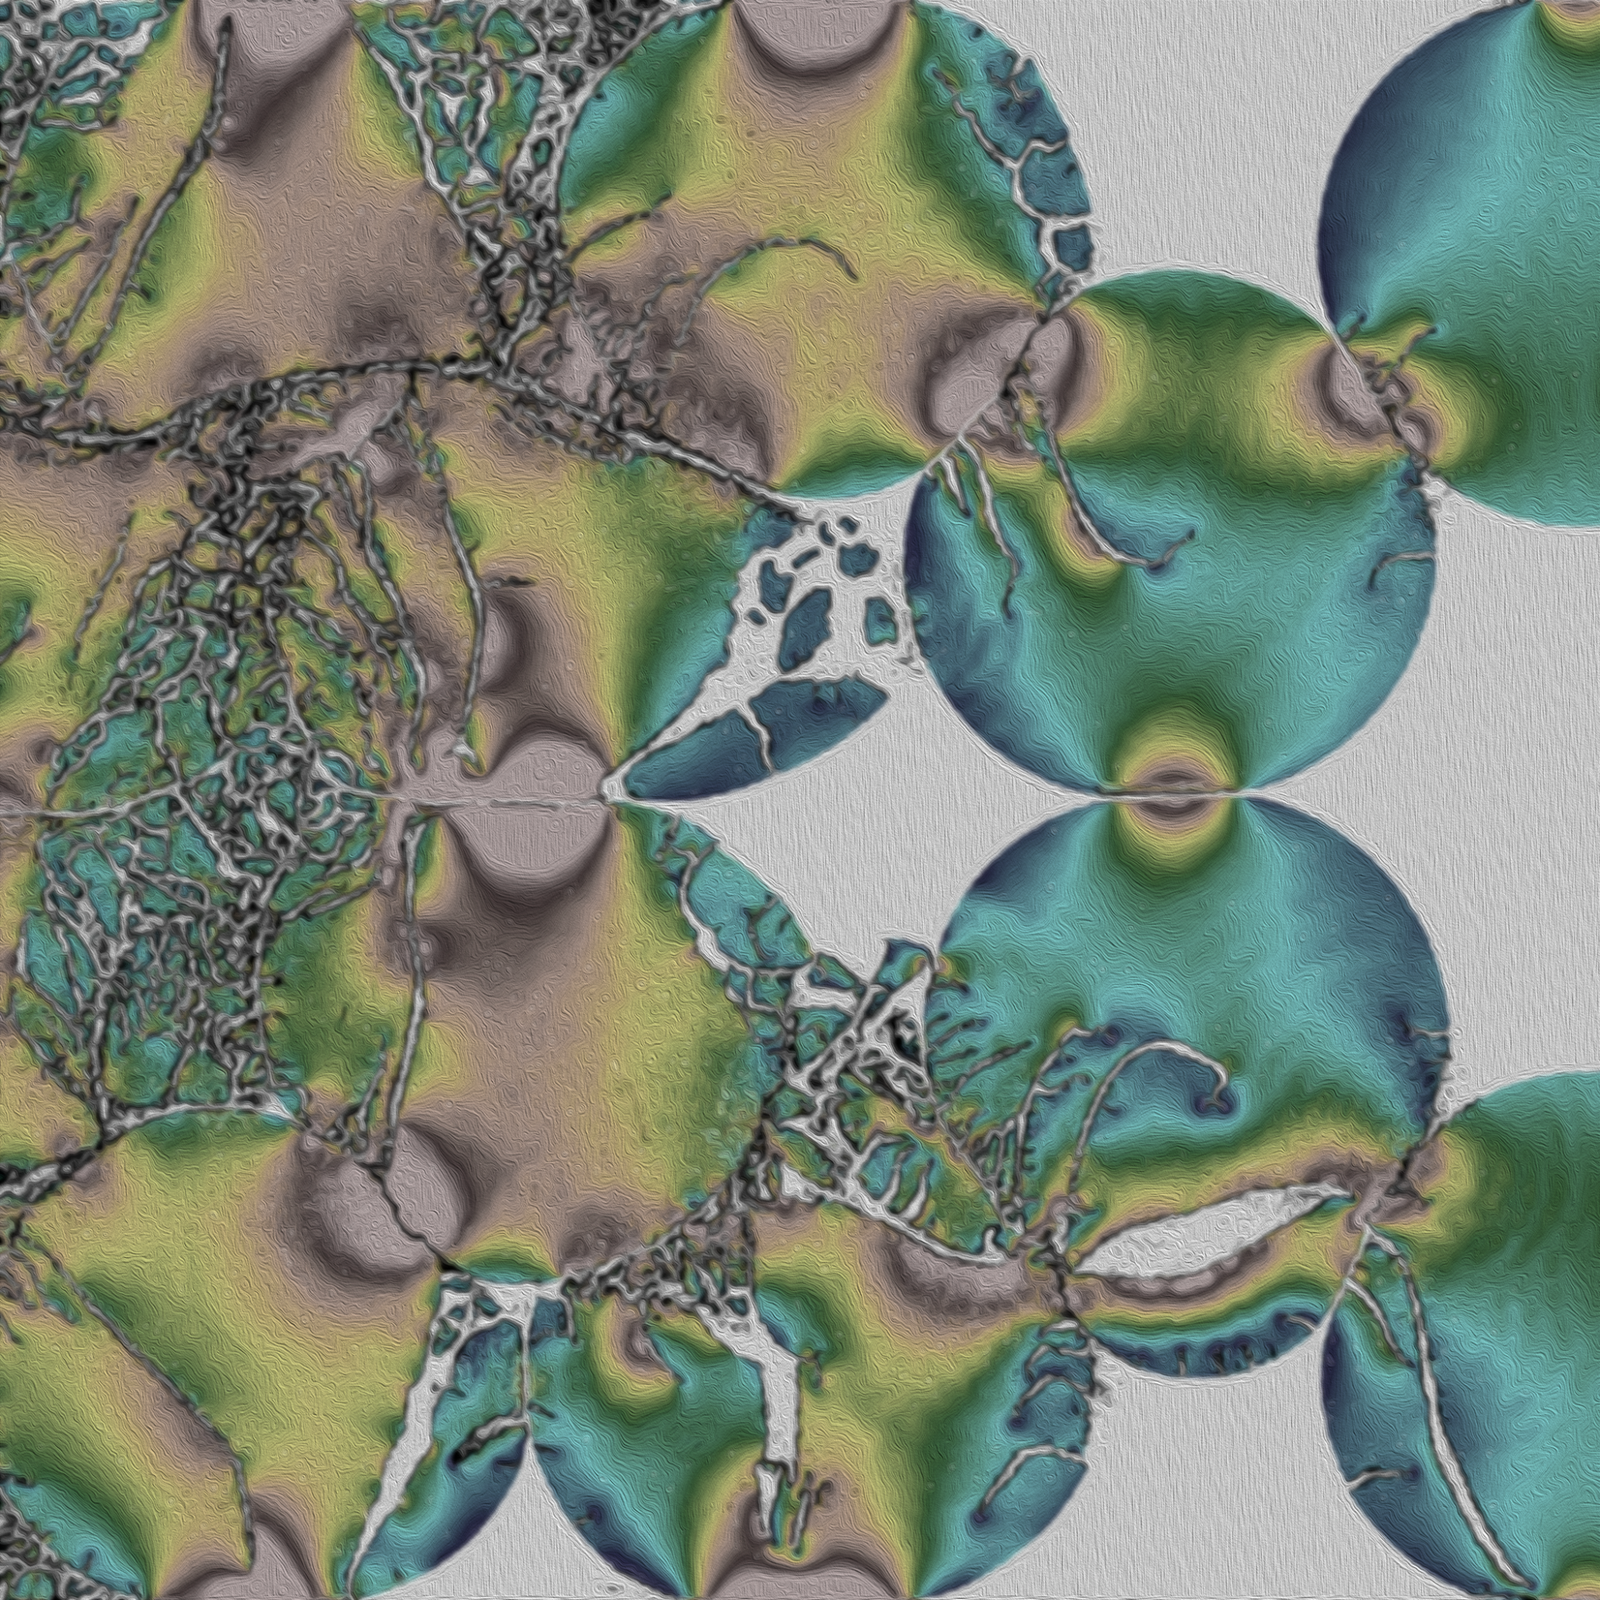
\includegraphics[height=0.32\textheight]{figures/cover_disk_compaction.png}\par
\vspace{0.45em}
{\footnotesize\emph{Stylized two-dimensional disk-compaction fragmentation result.}\par}
\vspace{0.55em}
\begin{minipage}{0.96\textwidth}
\footnotesize
\raggedright
\textbf{Core GEOS-MPM development}\par
Michael A. Homel, Ph.D. (LLNL) - GEOS-MPM LEAD Developer\par
Cameron M. Crook, Ph.D. (LLNL) - GEOS-MPM Developer\par
Stefan J. Povolny, Ph.D. (LLNL) - GEOS-MPM Developer\par
\vspace{0.35em}
\textbf{GEOS-MPM Contributors:}\par
Jay Appleton, Sohanjit Ghosh, Margariete Malenda, Jacob Nuttal\par
\vspace{0.35em}
\textbf{GEOS Infrastructure Support:}\par
Randy Settgast, Josh White, Matteo Cusini, Ben Corbett, Chris Sherman, Thomas Gazzola, Nicola Castalletto\par
\vspace{0.35em}
\textbf{Programmatic Support:}\par
Eric Herbold, Alan DeHope, Andrew Saab, Kyle Sullivan\par
\end{minipage}
\vfill
{\large Prepared by LLNL under Contract DE-AC52-07NA27344.\par}
\end{titlepage}
